\documentclass[12pt, a4paper]{article}
\usepackage[utf8]{inputenc}
\usepackage{amssymb}
\usepackage{indentfirst}
\usepackage{listings}
\usepackage{enumitem}
\usepackage{comment}
\usepackage{graphicx}
\usepackage{color}
\usepackage[portuguese]{babel}
\usepackage{geometry}
\geometry{legalpaper, a4paper,
 total={170mm,257mm},
 left=20mm,
 top=20mm}
\setlength{\voffset}{-10mm}
\definecolor{dkgreen}{rgb}{0,0.6,0}
\definecolor{gray}{rgb}{0.5,0.5,0.5}
\definecolor{mauve}{rgb}{0.58,0,0.82}

\lstset{frame=tb,
  language=Java,
  aboveskip=3mm,
  belowskip=3mm,
  showstringspaces=false,
  columns=flexible,
  basicstyle={\small\ttfamily},
  numbers=none,
  numberstyle=\tiny\color{gray},
  keywordstyle=\color{blue},
  commentstyle=\color{dkgreen},
  stringstyle=\color{mauve},
  breaklines=true,
  breakatwhitespace=true,
  tabsize=3
}

\newcommand{\tit}[1]{\textit{#1}}
\newcommand{\tb}[1]{\textbf{#1}}
\newcommand{\tbi}[1]{\textbf{\textit{#1}}}

\newcommand{\bitem}[2]{ \tb{(\tit{#1}) {#2}}}
\newcommand{\iitem}[1]{(\tit{#1})}

\newcommand{\oo}{orientação à objetos}
\newcommand{\sw}{\tit{software}}
\newcommand{\ssw}{\tit{software} }

\newcommand{\question}[1]{\item \tb{#1}}
\newcommand{\answer}[1]{\par \tb{Resposta:} #1}

\newcommand{\quotes}[1]{``#1''}

\title{Módulo 4 - Atividade Individual \\
  \large Análise de Software e UML}

\author{Wellington M. Espindula}
\date{Março de 2021}

\begin{document}
    \maketitle
    
    \begin{enumerate}[label=\textbf{\arabic*.}]
        % Question 1
        \question{Modelo Conceitual: Inscrição em Disciplinas. Identificar as classes de domínio para o caso de uso a seguir. Para cada classe identificada, relacionar os atributos, operações e associações que você conseguir identificar. Construir o diagrama de classes. (Fonte: Bezerra, E. Princípios de Análise e Projeto de Sistemas com UML 2.0)}
        \answer{
           \begin{figure}[ht!]
               \centering
               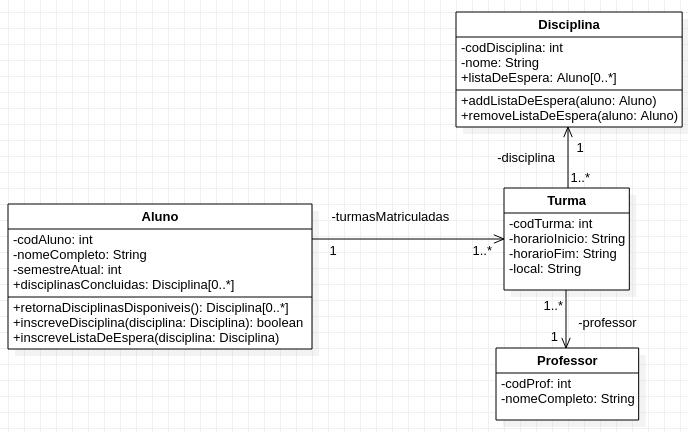
\includegraphics[width=0.85\textwidth]{quest1.png}
               \label{fig:quest1}
               \caption{Diagrama de Classes do sistema de inscrição em Disciplinas. Fonte: O Autor, 2021.}
           \end{figure} 
        } \newpage
        
        % Question 2
        \question{Casos de Uso – Loja de CDs. Faça o diagrama de casos de uso do seguinte enunciado. \\
            \normalfont{\tit {
                Um sistema permite o cadastramento de sócios e filmes, e a locação de filmes. Um filme tem obrigatoriamente ao menos uma cópia, mas pode possuir diversas delas, porém uma cópia refere-se exclusivamente a um determinado filme. Um sócio autonomamente se cadastrar e pode realizar muitas locações enquanto permanecer sócio da locadora, mas uma locação refere-se unicamente a um determinado sócio. Cada locação deve obrigatoriamente referenciar-se ao menos uma cópia de um filme, podendo referenciar-se a muitas cópias, no entanto uma cópia pode ter sido locada diversas vezes, em épocas diferentes.
            }}
        }
        \answer{
           \begin{figure}[ht!]
               \centering
               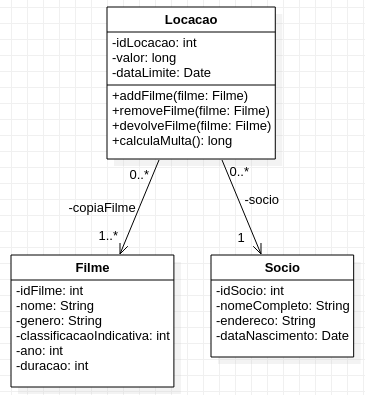
\includegraphics[height=0.45\textheight]{quest2.png}
               \label{fig:quest2}
               \caption{Diagrama de Classes da locação de filmes. Fonte: O Autor, 2021.}
           \end{figure} 
        } \newpage
        
        % Question 3
        \question{
            Modelo Conceitual: Venda de Produtos. Represente usando um diagrama de classes as INFORMAÇÕES a seguir.
            \normalfont{
                \begin{itemize}
                    \item A Firma Limpex vende produtos de limpeza, e deseja melhor controlar os produtos que vende, seus clientes e o os pedidos de seus clientes.
                    \item Cada produto é caracterizado por um código, nome do produto, categoria, e seu preço. A categoria é uma classificação criada pela própria firma (ex. detergente, sabão em pó, sabonete), e somente são vendidos produtos pertencentes a categorias previamente definidas.
                    \item A firma possui informações sobre todos seus clientes. Cada cliente é caracterizado por seu código interno, nome do cliente, endereço, um ou mais telefone, e o seu limite de crédito.
                    \item Registra-se a informação de todo e qualquer pedido feito por um cliente. Cada pedido possui um número, e guarda-se a data deste. Cada pedido envolve pelo menos um produto, e para cada produto, indica-se a quantidade deste pedida.
                \end{itemize}
            }
        }
        \answer{
           \begin{figure}[ht!]
               \centering
               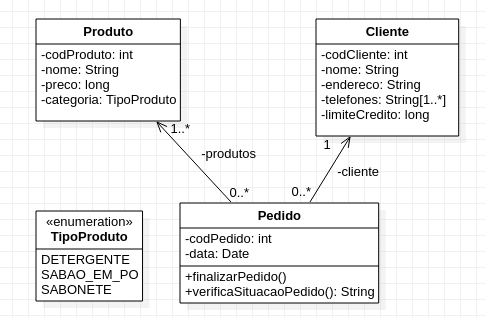
\includegraphics[width=0.85\textwidth]{quest3.png}
               \caption{Diagrama de Classes da Venda de Produtos. Fonte: O Autor, 2021.}
               \label{fig:quest3}
           \end{figure}
        }
        \newpage
        
        % Question 4
        \question{Represente estas informações em um diagrama de classes. \\
            \normalfont{\tit {
                BROLIWOOD possui diversos estúdios cinematográficos, cada um caracterizado por um nome, nome do(s) sócio(s), data de fundação, e o faturamento do ano anterior. Estes estúdios produzem filmes que possuem um nome, o número de meses que levou sendo feito, o ano de lançamento, custo total de produção do filme, e, quando for lançado, faturamento. Em cada filme atuam atores, que possuem um nome artístico, uma nacionalidade, idade, sexo, e um conjunto de tipos de papéis para o qual seu tipo físico é aconselhável (ex: avó, mocinha jovem, galã com idade avançada, adolescente). Estes tipos de papéis não são pré-definidos, constituindo uma lista preenchida a critério de cada ator para fins de casting. Em cada filme onde atua, um ator ganha um cachê, e desempenha um personagem que possui um nome. Estúdios podem existir mesmo que ainda não tiverem produzido um filme, mas só são considerados atores que já atuaram em pelo menos um filme. Só são registrados filmes já produzidos.
            }}
        }
        \answer{ \\
           \begin{figure}[ht!]
               \centering
               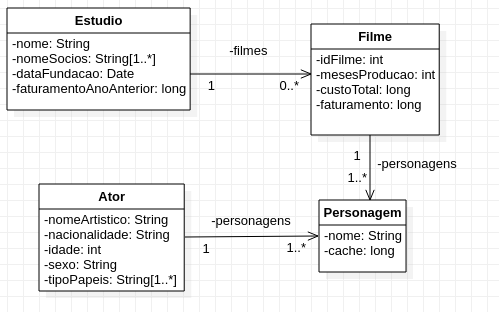
\includegraphics[width=0.85\textwidth]{quest4.png}
               \caption{Diagrama de Classes dos Estúdios Cinematográficos de Broliwood. Fonte: O Autor, 2021.}
               \label{fig:quest4}
           \end{figure}
        }
        \newpage
        
        
        % Question 5
        \question{Crie o diagrama de classes. \\
            \normalfont{\tit {
                Um aeroclube tem interesse em manter o controle sobre todos os seus sócios, bem como sobre as aulas práticas realizadas pelos seus alunos. \\
                Os sócios dividem-se em pilotos, instrutores e alunos de pilotagem. Todos sócios são caracterizados pelo número de matrícula, nome, endereço e idade. Os pilotos possuem um número de brevê. Os instrutores são pilotos com formação adicional de instrutor, devendo ser registrados o nome do curso de sua formação e a data de obtenção do diploma. A escola só ministra cursos básicos, e portanto não há pilotos ou instrutores que são alunos de cursos avançados. \\
                Alunos são sócios que seguem uma formação teórica-prática visando obtenção de um breve. Para estes alunos, deseja-se unicamente registrar todos os seus voos para contabilização de horas necessárias à obtenção do brevê. Para cada voo de um aluno, registra-se instrutor (deve ser um dos instrutores do clube), data, hora de saída e de chegada, bem como o parecer do instrutor sobre o voo.
            }}
        }
        \answer{\\
           \begin{figure}[ht!]
               \centering
               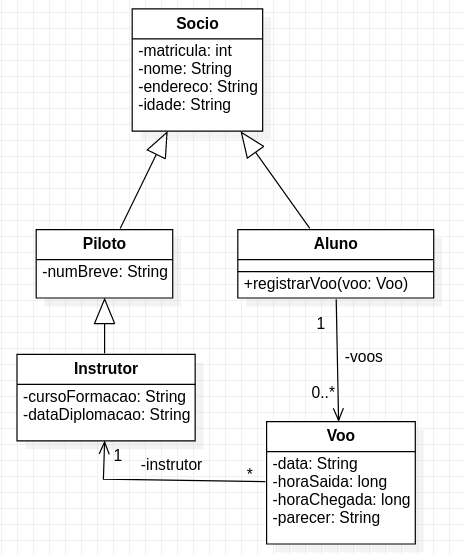
\includegraphics[height=0.55\textheight]{quest5.png}
               \caption{Diagrama de Classes do Aeroclube. Fonte: O Autor, 2021.}
               \label{fig:quest5}
           \end{figure}
        }
        \newpage
 
    
        % Question 6
        \question{Modelo Conceitual: Considere o enunciado do sistema de Biblioteca fornecido no módulo anterior e faça o seu modelo conceitual, representando-o através de um diagrama de classes.}
        \answer{  \\
           \begin{figure}[ht!]
               \centering
               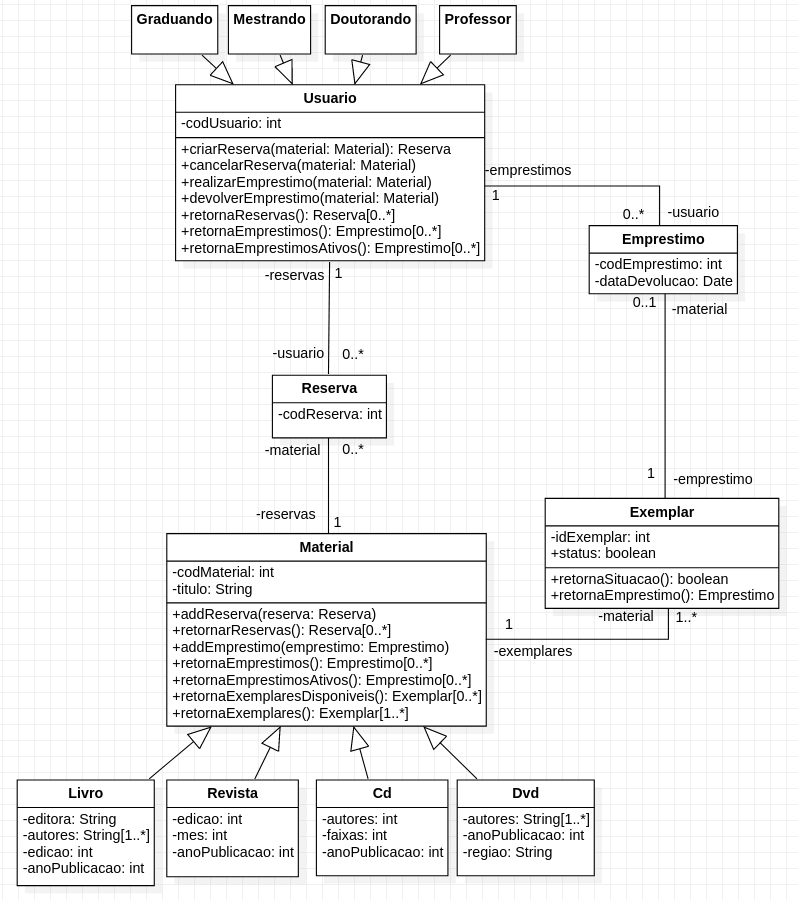
\includegraphics[width=0.85\textwidth]{quest6.png}
               \caption{Diagrama de Classes do sistema Biblioteca. Fonte: O Autor, 2021.}
               \label{fig:quest6}
           \end{figure}
        }
        \newpage
        
        
            
        % Question 7
        \question{Faça um diagrama de atividades correspondente, com atividades/ações e fluxo de execução (sequenciamento, pontos de decisão, paralelismo, pontos de sincronização, etc.). \\
        \normalfont{\tit {Confecção de um bolo: Maria procura a receita de um bolo. Quando encontrar, Evan mistura os ingredientes secos, enquanto Maria os ingredientes molhados. Ao mesmo tempo que os ingredientes molhados e secos são separadamente misturados, Helen deve aquecer o forno. Quando os ingredientes secos e molhados estiverem misturados “separadamente”, Evan deve misturá-los em um único recipiente. Após, o forno estar aquecido “e” todos os ingredientes misturados, Maria deve colocar o bolo para assar. Se o bolo estiver assado, Helen deve retirá-lo do forno, senão este deve continuar assando. }}
        }
        \answer{  \\
           \begin{figure}[ht!]
               \centering
               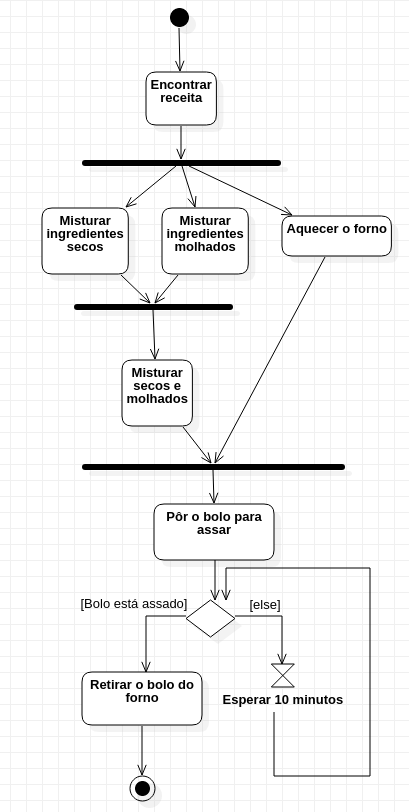
\includegraphics[height=0.7\textheight]{quest7.png}
               \caption{Diagrama de atividades da Confecção de um bolo. Fonte: O Autor, 2021.}
               \label{fig:quest6}
           \end{figure}
        } \newpage
        
                    
        % Question 8
        \question{Faça o diagrama de estados que representa o funcionamento do ATM abaixo descrito. \\
        \normalfont{\tit {O ATM está inicialmente desligado. Depois que ele é ligado, o ATM realiza uma ação de inicialização e entra em um estado de auto-teste. Se o teste falha, o ATM vai para um estado de fora de serviço, caso contrário tem uma transição sem trigger para um estado em espera. Neste estado, o ATM espera para a interação com o cliente. \\
        O estado do ATM muda do estado em espera para o estado de serviço ao cliente quando o cliente insere o cartão do banco ou de cartão de crédito no leitor de cartão do ATM. Quando entra no estado de serviço ao cliente, a ação de entrada lerCartão é executada. Note que a transição do estado de serviço ao cliente de volta para o estado em espera pode ser disparada pelo cancelamento do evento já que o cliente pode cancelar a transição a qualquer momento. \\
        O estado de servindo ao cliente é um estado composto com sub-estados seqüenciais: Autenticação do Cliente, Selecionando Transação e Transação. Autenticação do Cliente e Transação são também estados compostos, não detalhados neste diagrama. O estado de serviço ao cliente também tem uma transição sem trigger de volta para o estado em espera depois que a transação termina. O estado também tem uma ação de saída ejetarCartão que libera o cartão do cliente quando sai do estado, não importando o que causou a transição de saída do estado.}}
        }
        \answer{  \\
           \begin{figure}[ht!]
               \centering
               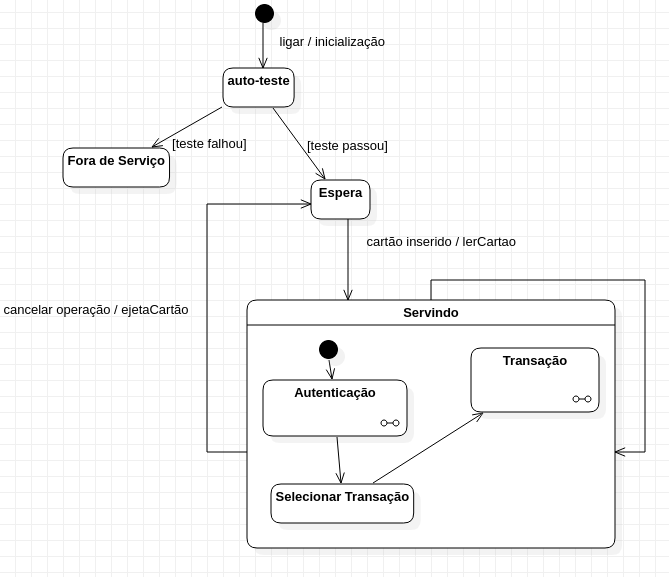
\includegraphics[width=0.85\textwidth]{quest8.png}
               \caption{Diagrama de estados do funcionamento da ATM. Fonte: O Autor, 2021.}
               \label{fig:quest6}
           \end{figure}
        }
    \end{enumerate}



    
\end{document}